\chapter{Introduction}

%\begin{quote}
%\lipsum[1]
%\end{quote}
\section{Lasers for Particle Acceleration}

Explain what a laser stands for, stimulated emission, lasing medium, what the Ti:sapphire crystal does and why it is chosen, CPA

\subsection{Chirped Pulse Amplification}

\subsection{...}

%In this template, the acronyms are all placed in a separate file called
%\verb#acronmys.tex# which is then loaded with \verb#%A list of common acronyms
%Only those used will be displayed, so you can just add to this list
\newacronym{LLNL}{LLNL}{Lawrence Livermore National Laboratory}
\newacronym{LANL}{LANL}{Los Alamos National Laboratory}
\newacronym{NIF}{NIF}{National Ignition Facility}
\newacronym{NIF-ARC}{NIF-ARC}{National Ignition Facility - Advanced Radiographic Capability}
\newacronym{OMEGA-EP}{OMEGA-EP}{OMEGA Extended Performance System}
\newacronym{RF}{RF}{radio frequency}
\newacronym{QCD}{QCD}{quantum chromodynamics}
\newacronym{QED}{QED}{quantum electrodynamics}
\newacronym{WKB}{WKB}{Wentzel-Kramers-Brillouin}
\newacronym{SRIM}{SRIM}{stopping range of ions in matter}
\newacronym{SOBP}{SOBP}{spread-out Bragg peak}
\newacronym{OSUCCC}{OSUCCC}{The Ohio State Comprehensive Cancer Center}
\newacronym{LLE}{LLE}{Laboratory for Laser Energetics}
\newacronym{TNSA}{TNSA}{target normal sheath acceleration}
\newacronym{IBA}{IBA}{Ion Beam Analysis}
\newacronym{IMPT}{IMPT}{intensity modulated proton therapy}
\newacronym{ALLS}{ALLS}{Advanced Laser Light Source}
\newacronym{XPIF}{XPIF}{x-ray and particle-induced fluorescence}
\newacronym{EDX}{EDX}{energy dispersive x-ray fluorescence}
\newacronym{TEM}{TEM}{transverse electromagnetic mode}
\newacronym{FWHM}{FWHM}{full width at half maximum}
\newacronym{eTNSA}{eTNSA}{enhanced target normal sheath acceleration}
\newacronym{LWFA}{LWFA}{laser wakefield acceleration}
\newacronym{PIC}{PIC}{particle-in-cell}
\newacronym{NGP}{NGP}{nearest grid point}
\newacronym{CCD}{CCD}{charge coupled device}
\newacronym{RPA}{RPA}{radiation pressure acceleration}
\newacronym{LSP}{LSP}{Large Scale Plasma: An implicit particle-in-cell code}
\newacronym{NN}{NN}{neural network model}
\newacronym{SVGP}{SVGP}{stochastic variational gaussian process}
\newacronym{GPR}{GPR}{gaussian process regression}
\newacronym{POLY}{POLY}{polynomial regression}
\newacronym{ML}{ML}{machine learning}
\newacronym{AI}{AI}{artificial intelligence}
\newacronym{HEDS}{HEDS}{high energy density science}
\newacronym{BO}{BO}{bayesian optimization}
\newacronym{WP-ELL}{WP-ELL}{Extreme Light Laboratory at the Wright-Patterson Air Force Base}
\newacronym{GPU}{GPU}{Graphics Processing Unit}
\newacronym{OSC}{OSC}{Ohio Supercomputer Center}
\newacronym{SVR}{SVR}{Support Vector Regression}
\newacronym{RBF}{RBF}{Radial Basis Function}
\newacronym{MAPE}{MAPE}{Mean Absolute Percentage Error}
\newacronym{MSE}{MSE}{Mean Squared Error}
\newacronym{RMSE}{RMSE}{Root Mean Squared Error}
\newacronym{AFIT}{AFIT}{Air Force Institute of Technology}
\newacronym{CSUCI}{CSUCI}{California State University - Channel Islands}
\newacronym{CSU}{CSU}{Colarado State University}
\newacronym{RAL}{RAL}{Rutherford Appleton Laboratory}
\newacronym{DAQ}{DAQ}{Data Acquisition System}
\newacronym{OAP}{OAP}{off-axis parabolic mirror}
\newacronym{HDF5}{HDF5}{Hierarchical Data Format 5}
\newacronym{EPICS}{EPICS}{Experimental Physics and Industrial Control System}
\newacronym{GUI}{GUI}{Graphical User Interface}
#, to
%make the main source file easier to read.  You can also just put all
%your acronyms directly in the header of your main source file.
%
%Once you have defined an acronym, you can use it with the \verb#\gls{<label>}# command.
%The first time you use the acronym, the full definition is printed: atomic force microscopy (AFM). %\gls{AFM}.
%On subsequent uses, just the abbreviation is printed: AFM %\gls{AFM}
% - Latex keeps track
%for you, so you don't have to do this manually.  There are fancier forms
%of \verb#\gls# that allow you to capitalize (\verb#\Gls{<label>}#) or use the 
%plural (\verb#\glspl{<label>}#) forms of your abbreviations.  See 
%for example \url{http://en.wikibooks.org/wiki/LaTeX/Glossary} for details
%on the glossaries package.

%If you want to list all your acronyms at the beginning of your document, you
%will need to include the \verb#\makeglossaries# command in your preable, as
%shown above, and then 
%\begin{verbatim}
%\printglossary[type=\acronymtype]
%\end{verbatim}
%where you want the list of abbreviations to actually appear 
%(as stated above, this must be right after your lists of figures and tables in the roman
%numeral pages at the beginning of the document).  Then you have
%to go to the terminal (in the directory containing your document), and run the command
%\begin{verbatim}
%makeglossaries (yourdocumentname)
%\end{verbatim}
%to actually create the glossary.  If you just want Latex to keep track of your acronyms for you 
%and print no list, you can just skip this step and the \verb#printglossary# command.

%To make the heading for the List of Abbreviations look the same as the List of Figures
%and List of Tables, instead of using \verb#\printglossary# I defined a custom command to print the glossary:
%\begin{verbatim}
%\newcommand\PrintListofAbbreviations[1]{
%\phantomsection
%\addcontentsline{toc}{front}{\typesetColumnHeading{#1}}
%\printglossary[type=\acronymtype,title={\protect {\typesetLevelTwo{#1}}}]
%%\end{verbatim}
%This command functions the same as \verb#\printglossary#, but instead
%of typesetting the heading like a chapter heading (in smallcaps), 
%it typesets in bold like the lists of figures and tables.  
%To use it, just call \verb#\PrintListofAbbreviations{List of Abbreviations}#
%right after \verb#\listoftables# and before \verb#\mainmatter#.
%If you wish to use a different title for you list of abbreviations,
%just call \verb#\PrintListofAbbreviations{Your Title}#.
%I am unsure if the GS has any restrictions on what title you can use.
%
%One final comment, this template uses \verb#makeindex# to create the glossaries
%for compatability (some versions of Ubuntu for example don't support \verb#xindy#).
%However, there is a better program for making glossaries that you can use by calling
%\begin{verbatim}
%\usepackage[xindy,toc,acronym, section=chapter]{glossaries}
%\end{verbatim}
%instead.  In particular, \verb#xindy# allows you to use symbols in your abbreviations,
%such as Greek letters or accented characters, which are not supported by \verb#makeindex#.
%
%This figure also illustrates the use of subfigures via the subfig package, loaded by placing 
%\verb#\usepackage{subfig}# in the preamble of \verb#template.txt#.  This allows you to include
%each subfigure as an individual image, and have latex arrange and label them for you 
%(including an optional name for each subfigure in \verb#[]#).  This also allows
%you to individually reference Fig.~\ref{one_battery} and Fig.~\ref{five_battery}.
%Note that many journals DO NOT support this, and require that each figure be a single
%image, but this should be fine for a thesis.  
%
%A footnote\footnote{Another foot.}

\section{Applications}

This section highlights some of the most important applications of laser-based proton accelerators that motivates much the projects I have worked in during my PhD studies: (1) proton therapy for cancer treatment, (2) proton radiography for imaging, and (3) ion beam analysis for materials characterization.


\subsection{Proton Therapy}

Due to having no cure, cancer is one of the largest medical challenges faced worldwide and generally requires the use of harsh treatments like invasive surgery, chemotherapy, and immunotherapy. Another relevant treatment is called radiotherapy and more than half of all people with cancer will receive it as a part of their medical care \cite{Mayo_2024_Cancer}. Typically, a large machine will provide a source of x-rays (a type of energetic ionizing radiation) that kills the tumor. However, this radiation does not discern whether the cells are cancerous or not -- healthy tissue along the radiation beam path surrounding the tumor will also be damaged. This damage can be mitigated by shooting many beams from different angles such that they overlap at the site of the tumor. In this way, the dose delivered in the beam overlap region will be significantly higher than the surrounding tissue. This approach is typically employed by situating the machine on a rotating ``gantry''

As early as 1905, Bragg \cite{Bragg_1905_JOS} identified that charged particles have different properties than x-rays when passing through matter. Specifically, he identified that radium particles lost more energy (i.e. delivered a higher dose) at a lower speed. Physically, the slower the radium particles, the more time it has to interact with each of the individual atoms and the more energy it can deposit. This means that when the radium first enters a material at its highest speed, it is losing energy slowly in contrast to when it is at a slow speed and about to stop it is losing energy very quickly. In 1946, Wilson \cite{Wilson_1946_Rad} identified that this property of charged particles would enable a more concentrated dose to be delivered closer to the site of a tumor. In \autoref{fig:bragg_curve}, these differences are explicitly highlighted between x-rays and proton beams traveling through water. It can be seen that the proton beam is sharply peaked at a particular distance of around 23 centimeters, where the x-ray beam delivers a relatively higher dose at just a few centimeters. One can see the advantage of protons quite readily from this picture -- if a tumor is located 23 centimeters into the body, the protons, comparatively to the x-rays, will deliver more energy at the tumor site and less energy to the surrounding tissue. The shape of the proton beam curve in this graph is appropriately referred to as a ``Bragg Curve'' which peaks at the ``Bragg Peak''. 

The specifics of the depth-dose curve depend on the material that the particles are traveling through as well as initial energy of the protons. These conditions are well-studied by empirical measurements of the \gls{SRIM} \cite{Ziegler_2010_SRIM} and can be combined with other techniques to achieve a depth-dose curve that not only peaks at different depths, but also has a \gls{SOBP} that expands the region where the highest dose is delivered. The most modern form of proton therapy is called \gls{IMPT} whose intensities are modulated to optimally balance tumor dose and sparing of normal tissues \cite{Mohan_2022_PRO}. The first proton therapy center opened at the Loma Linda University Medical Center in California in 1990, but today there are more than 100 centers around the world with more that are planned or in the process of construction \cite{Mohan_2022_PRO}. 

\begin{figure}
	\centering
	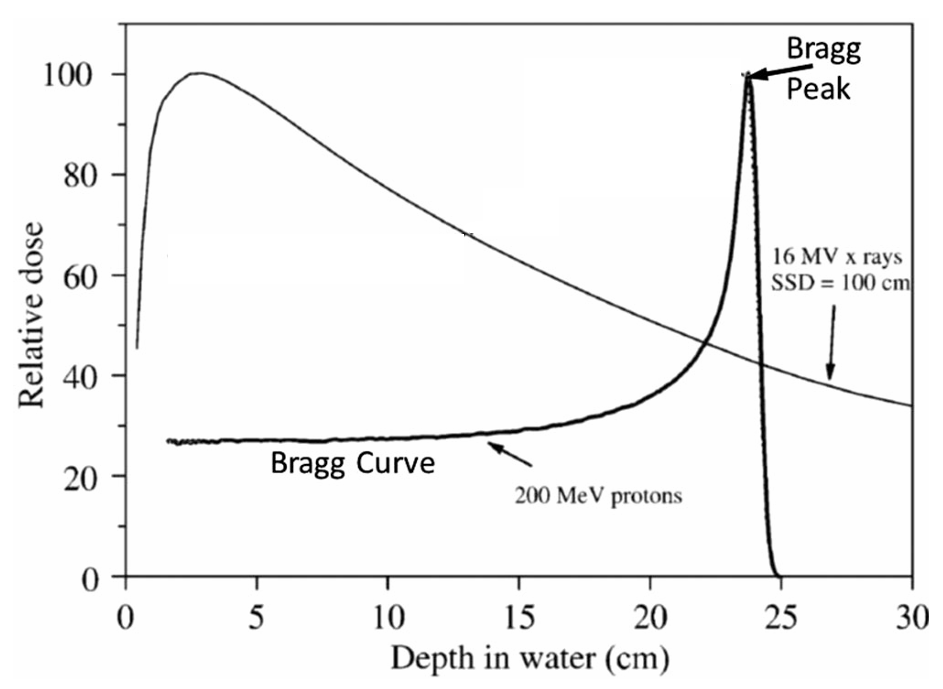
\includegraphics[width=0.75\linewidth]{planning/images/bragg_curve.PNG}
	\caption{The dose delivered as a function of depth traveled in water for two types of beams are depicted -- 200 MeV protons and 16 MV x-rays. Taken from Figure 1 in Mohan \cite{Mohan_2022_PRO}.}
	\label{fig:bragg_curve}
\end{figure}
 
Right here in Columbus, \gls{OSUCCC}, in collaboration with Nationwide Children's Hospital opened a 55,000 square foot proton therapy center in December of 2023 \cite{OSU_CCC} that uses \gls{IMPT}. Despite all the aformentioned benefits of proton therapy, the intial cost is tremendous -- \gls{OSUCCC} was a 100 million dollar investment. The significant cost demonstrates the value this could bring to Central Ohio. The facility is even outfitted with the capability to perform FLASH therapy -- a newer, experimental form of proton therapy that can be delivered in seconds that is still in clinical trials \cite{OSU_CCC} -- which shows the continued investment and innovation in this field. 

The cost, however, cannot be overlooked. The conventional cyclotron accelerators used to accelerate the protons are extremely large and expensive. In recent years, it has been proposed that laser-based particle accelerators could be used to generate high energy protons. These facilities could in principle be smaller and less costly, but the technology is not adequately matured to be considered in the near future \cite{Linz_2016_LaPB}. Laser-based sources are typically only able to generate protons in the 10s of MeV reliably (as opposed to the 100s of MeV required for clinical operation), possess orders of magnitude smaller numbers of protons, and poor reproducibility of the laser pulse output. In addition, the conventional accelerators have already made significant strides in terms of reducing cost, increasing beam quality, and reducing size in recent years \cite{Linz_2016_LaPB} which is something laser-based sources will need to keep up with in the future. However, the potential of developing a smaller and lower cost proton accelerator remains an important motivating factor for many laser-plasma physicists for the coming years.

\subsection{Proton Radiography and Laser Fusion}

All of us are familiar with the use of visible light to image things. A camera's flash will send out a burst of light and the camera will record the light reflected off an object to image it. Other frequencies of light not visible to the naked eye are used all the time to image things as well. High frequency sources like x-rays are used at the dentist due to their ability to probe matter within your body. Radio waves reflect well off of electrically conductive materials like the metals in vehicles which make them ideal for military applications. In an similar way, particles can be used to image objects by analyzing how they interact. Electron microscopes have been used extensively in the past century to image materials at a much higher resolution than an ordinary visible light microscope. From \autoref{fig:bragg_curve}, we know that protons interact with matter in a different way than electromagnetic radiation like x-rays. These differences can be exploited to image things that cannot be done well with other types of radiation \cite{Schaeffer_2023_RevMod}. To give one example, a proton is a charged particle that gets deflected by electric and magnetic fields which can enable scientists to obtain information about these fields in a way that x-rays cannot.

\begin{figure}
	\centering
	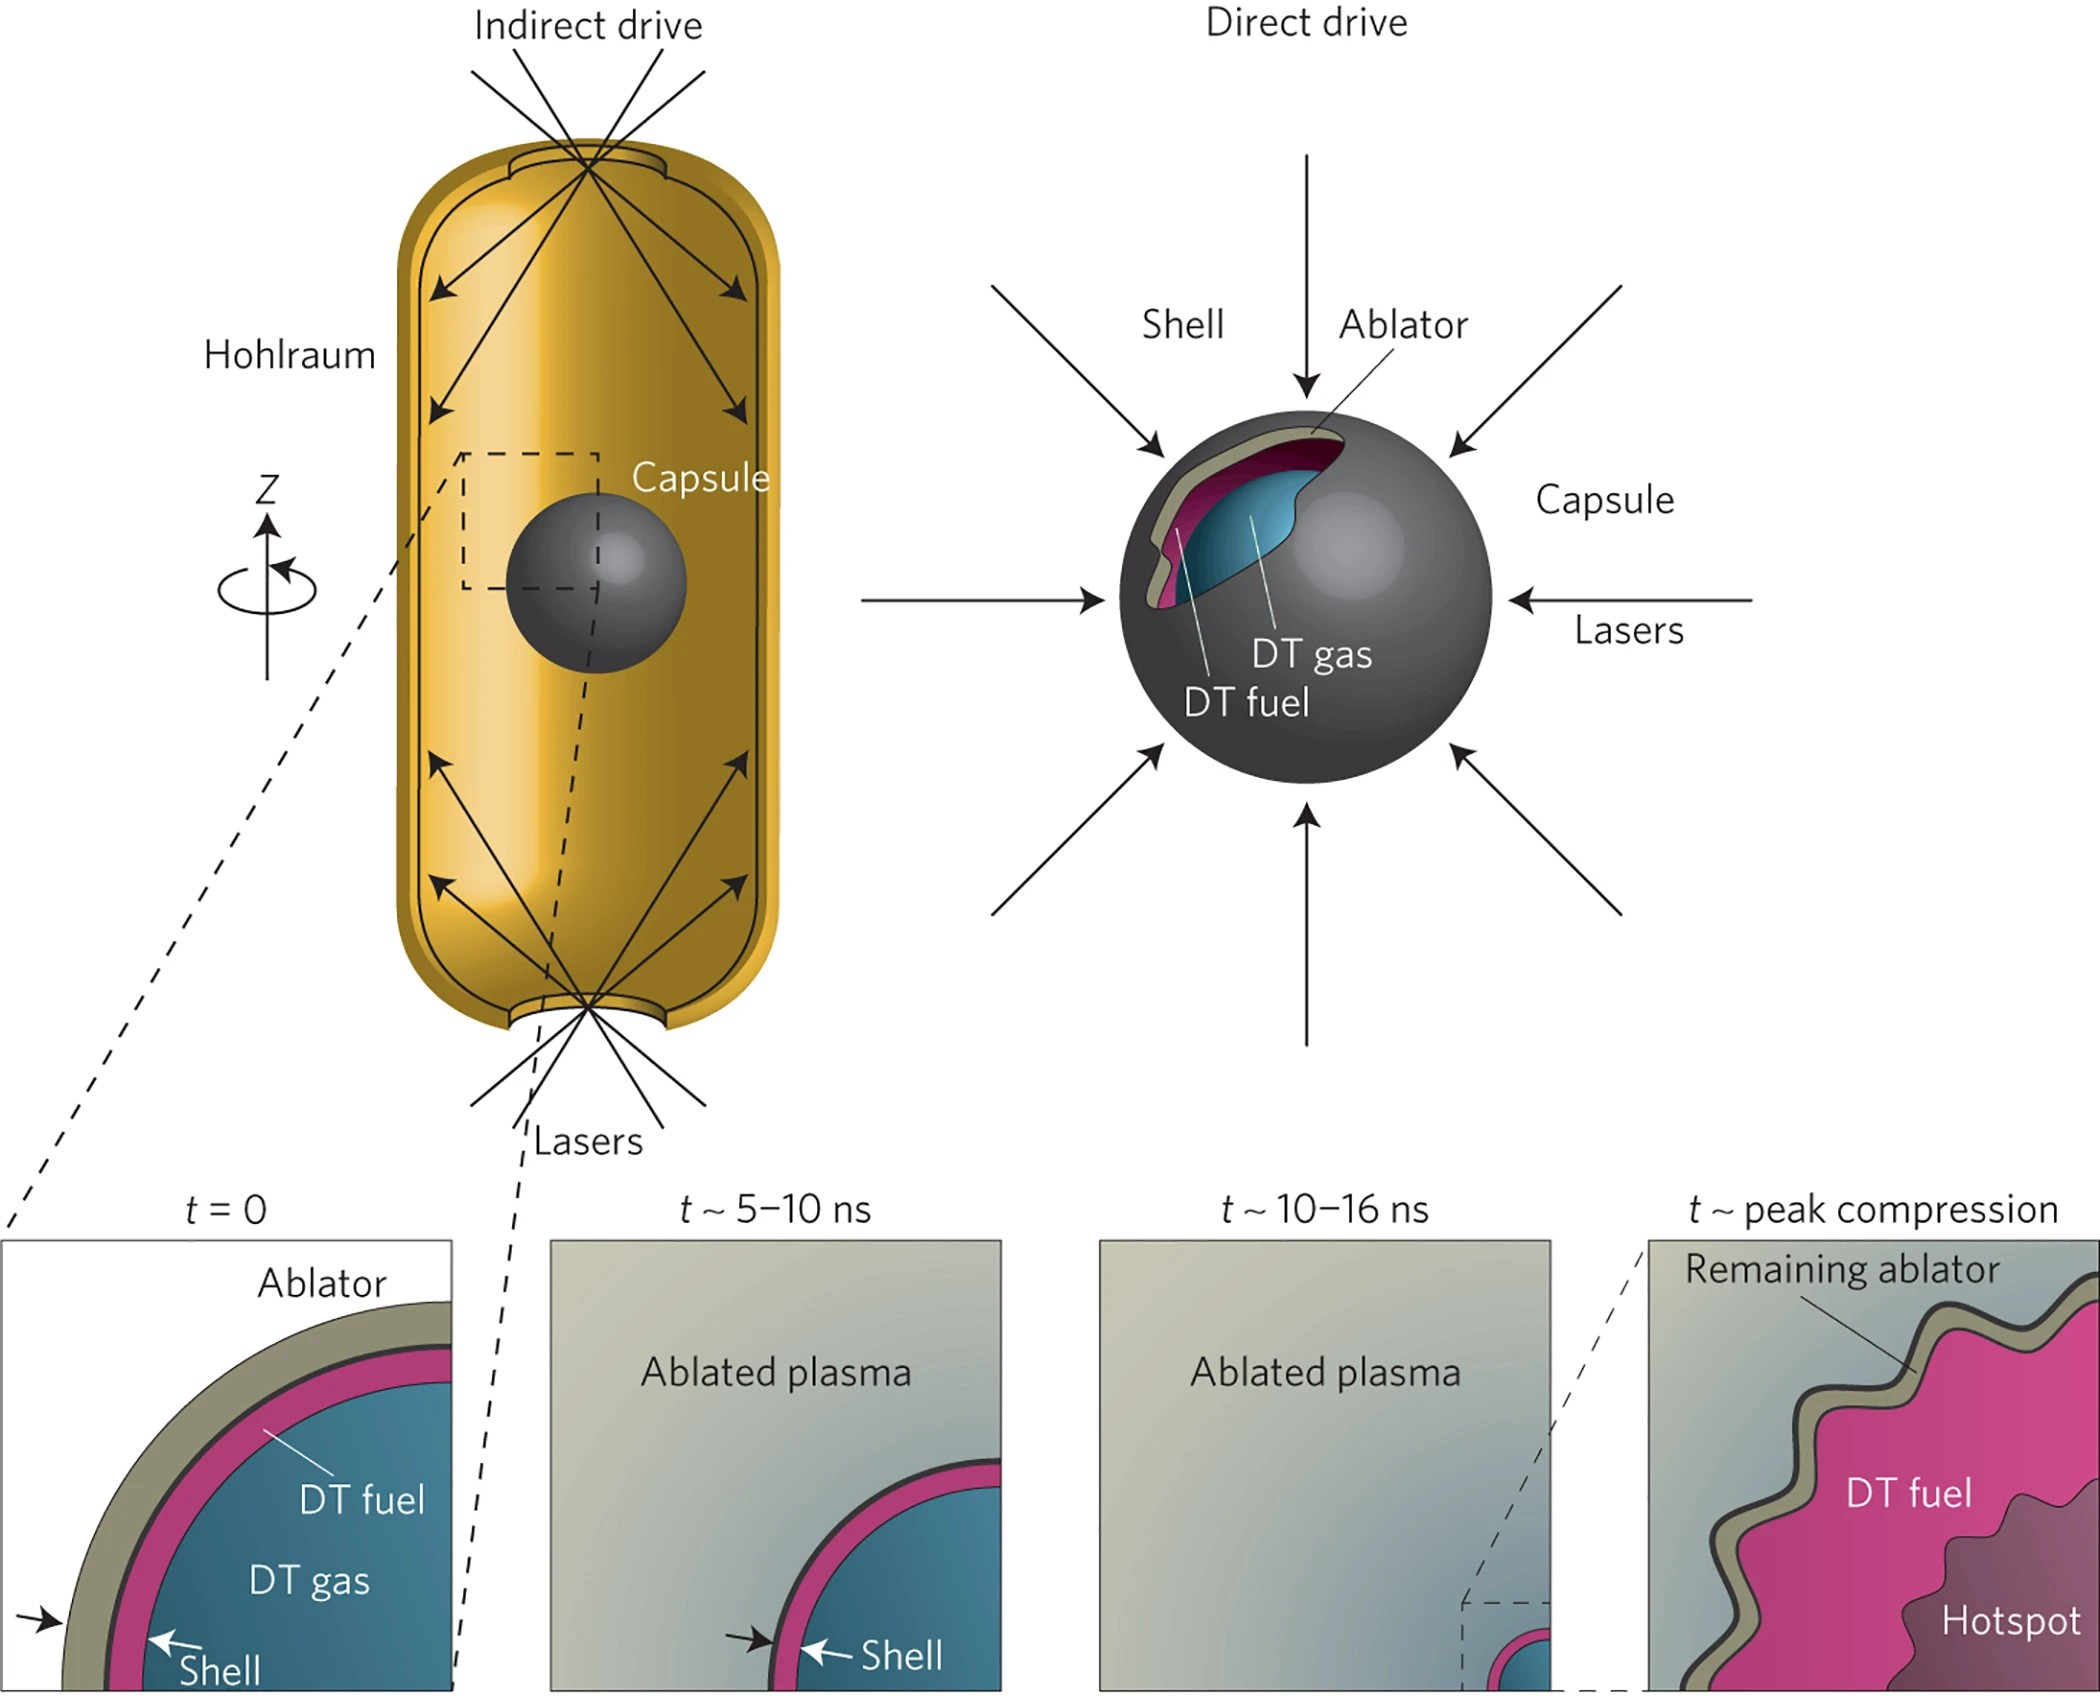
\includegraphics[width=0.75\linewidth]{planning/images/fusion.png}
	\caption{Visualization of two different approaches to laser fusion are depicted at the top. Lasers can irradiate the inside of a hollow gold can (called a hohlraum) to indirectly heat a fusion capsule or instead directly heat it. At the bottom, multiple stages of the fusion process are depicted including capsule ablation, compression, and burn. Taken from Figure 1 of Betti et al. \cite{Betti_2016_Nature}. }
	\label{fig:inertial_fusion}
\end{figure}

One example of proton radiography using laser-accelerated protons is through the \gls{NIF-ARC}. As it's name implies, \gls{NIF-ARC} is typically used as light source to collect radiograph images of laser fusion experiments at NIF. These fusion experiments involve using a high powered lasers to compress a millimeter sized frozen pellet of hydrogen fuel (specifically, heavier isotopes of hydrogen called deuterium and tritium) to such high temperatures and pressures that the atomic nuclei fuse together into helium. The sun is an example of a high temperature and pressure environment that is able to sustain fusion as its vast source of energy, but we must be a little bit more clever on Earth to obtain conditions like that of in the core of our sun. A similar capability to NIF-ARC exists at the \gls{LLE}'s \gls{OMEGA-EP}. The \gls{OMEGA-EP} provides diagnostics for the main OMEGA laser which performs fusion experiments by directly irradiating a fusion pellet. This is in contrast to the \gls{NIF} which indirectly compresses a fusion pellet by first irradiating a gold can that surrounds the pellet. These approaches are aptly called indirect and direct drive fusion and are depicted in \autoref{fig:inertial_fusion}. Proton radiography has been demonstrated successfully at the \gls{NIF} through \gls{NIF-ARC} \cite{Simpson_2021_PPCF} and at OMEGA through \gls{OMEGA-EP} \cite{Zylstra_2012_RSI} through \gls{TNSA} proton beams produced from laser-irradiated metallic foils.

Conventional sources of protons for radiography purposes are from linear accelerators like the pRad at \gls{LANL}. \gls{LANL} uses \gls{RF} waves of around 200 MHz to accelerate particles up to 800 MeV (SOURCE). The limitation of conventional \gls{RF} accelerators is the relatively low frequency. If we take the reciprocal of 200 MHz, we find that the separation between individual waves (the period) is around 5 nanoseconds. This may seem like a short time, but on the scale of femtosecond and picosecond ultra-intense pulses, this is a thousand or a million times longer! If one wanted to take proton radiographs of some experiment happening on a picosecond timescale, the conventional accelerator would not work. On the other hand, lasers typically used for laser-plasma experiments are in the infrared and have wavelengths of around 1 micron. A quick calculation tells us that the period is only around 3 femtoseconds. Since the lasers are pulsed at 3 femtoseconds, the emitted protons would also be pulsed at 3 femtoseconds which would theoretically allow us to capture 1 proton radiograph every 3 femtoseconds. Another advantage of these laser-accelerated proton beams is that they are emitted from a very small spot, on the order of microns, which is beneficial for obtaining a higher quality image \cite{Schaeffer_2023_RevMod}.

\subsection{Materials Characterization}

While protons can generate images through radiography, they can also more generally tell us information about materials as a whole through a process called \gls{IBA}. \gls{IBA} allows scientists to probe material composition and surface structures with MeV ion beams which are appealing partly due to their non-destructive nature (comparatively to sources like x-rays) \cite{Passoni_2019_SciRep}. \gls{IBA} is currently implemented through old Van de Graaf and Tandem accelerator technology, but Passoni \cite{Passoni_2019_SciRep} argues that \gls{TNSA} proton beams can achieve the same result in a more compact, portable, and cheaper setup.

\begin{figure}
	\centering
	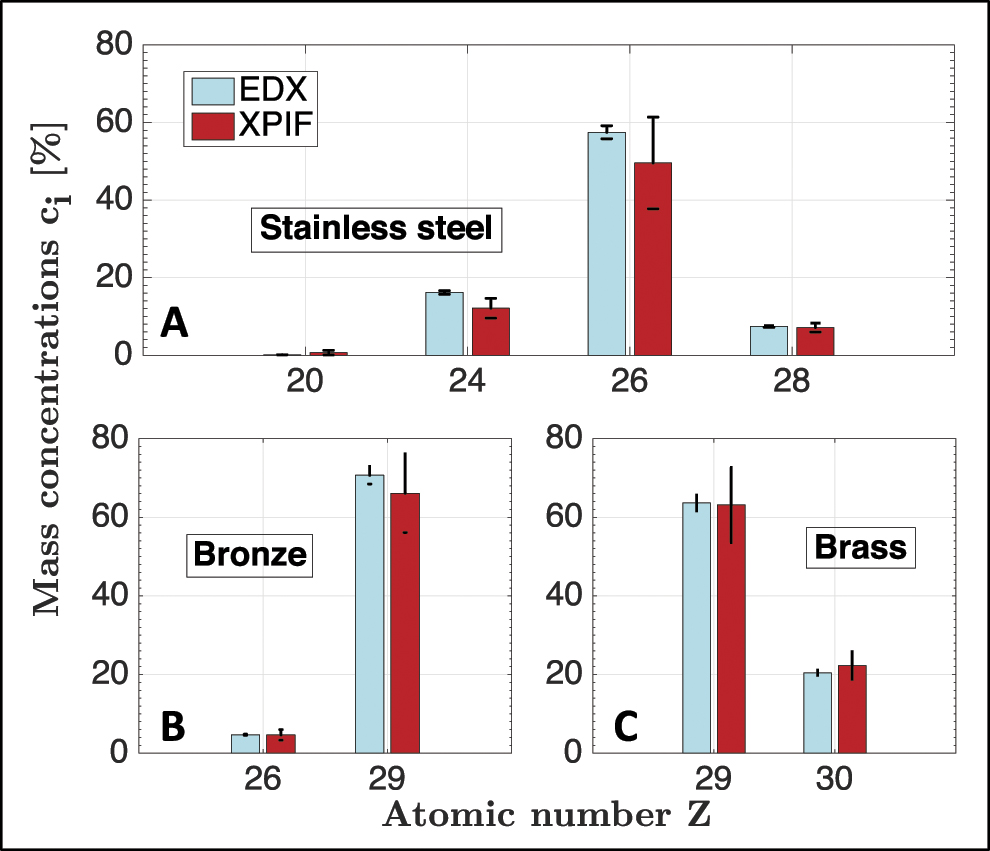
\includegraphics[width=0.6\linewidth]{planning/images/mass_concentration.jpg}
	\caption{Mass concentrations of three metal alloys are shown using two different techniques: energy dispersive x-ray (EDX) fluorescence and x-ray and particle-induced fluorescence (XPIF). Taken from Figure 4 of Boivin et al. \cite{Boivin_2022_NJoP}.}
	\label{fig:mass_concentration}
\end{figure}

As a proof of principle, Boivin \cite{Boivin_2022_NJoP} used TNSA beams from the ALLS laser facility in Canada to perform x-ray and particle-induced fluorescence (XPIF) to determine the elemental mass concentrations of three different metal alloys: stainless steel, bronze, and  brass. This is compared to a method called energy dispersive x-ray (EDX) fluorescence used in conjunction a conventional mono-energetic electron beam and shown in \autoref{fig:mass_concentration}. Although XPIF has larger error bars than EDX, both methods find good agreement with each other.

As a final point, TNSA beams can be accompanied by other radiation sources like electrons, x-rays, and neutrons. Different materials characterization process could, in principle, be used in conjunction with each other. While TNSA beams are not the most common way to characterize materials today, they may emerge as an important tool for their ability to be pulsed at a high repetition rate and generated from a relatively compact system.

\section{This Work}
Talk about prior work 


Talk about motivating question 


Talk about how work is organized. 


